\section{Design}
\subsection{Type checking background}
A type system consists of two major component: 1) \textit{types}, and 2) \textit{subtyping rules}.
A \textit{type} serves as an abstraction for the set of acceptable values for any expression. A \textit{type system} consists
\textit{types} that form a lattice of finite height. The hierarchy of types in this lattice defines subtyping relationships among them.
In our type system, we require every type hierarchy to define a unique \textit{@Top} and a \textit{@Bottom} element. This ensures that
any given pair of types has a \textit{least upper bound} and a \textit{greatest lower bound}.
Throughout this paper, we use the notation $@A <: @B$ to denote that type $@A$ is a subtype of type $@B$.
As an illustration of the type hierarchy, consider the lattice of types as shown in Figure~\ref{fig-example-lattice}.

\begin{figure}
	\begin{center}
		\includegraphics[scale=0.15]{lattice}
	\end{center}
	\caption{Example type hierarchy}
	\label{fig-example-lattice}
\end{figure}

example lattice
assignment, return examples
method overriding
collections type parameters
covariant, contravariant, and invariant subtyping

type hierarchy, subtype checking, Dataflow analysis rules, polymorphism

\subsection{Determinism type hierarchy}
Diagram of type hierarchy and explanation
Examples of errors produced when subtyping rules are violated (here)

The Determinism type system uses the following type qualifiers (see Figure~\ref{fig-determinism-hierarchy}):
\begin{itemize}
	\item $@NonDet$ indicates
	that the expression might have different values in two different executions on the same machine.
	\item $@OrderNonDet$ indicates that
	a collection (i.e any class that is a subtype of java.util.Collection or java.util.Iterator) or an array will have the same elements in every execution, but in a
	possibly different order.  $@OrderNonDet$ may only be written on
	collections and arrays.
	\item $@Det$ indicates that
	the expression evaluates to the same value (with respect to $.equals()$) in all
	executions on the same machine; for a collection, iteration also yields the values in the same
	order.
	This is the default qualifier.
\end{itemize}

\begin{figure}
	\begin{center}
		\includegraphics[scale=0.5]{determinism}
	\end{center}
	\caption{Determinism type hierarchy}
	\label{fig-determinism-hierarchy}
\end{figure}

\subsection{Additional typing rules for collection elements}
Lists, set and maps - element types have to be subtypes of collection type 
Explain iterator and extracting elements of an ordernondet collection here
Examples of valid and invalid types

\subsection{Avoid aliasing unsoundness}
Give an example of unsoundness 
Recall CLIMB-to-top rule and defaulting choice for local collections (to avoid too many warnings)
Required user annotations for collections and arrays

\subsection{Special cases of polymorphism}
Explain polymorphism first
Explain modifiers to Polymorphic annotations
Poly up and down for ordernondetermistic types
Poly use for avoiding polluting det/ordernondet collections
Subtype hierarchy among all variants of Poly
Possibility of type refinement?	

\subsection{Discussion on defaulting rules}
Choice of defaults on class type, constructors and method params and return types

\subsection{Additional hardcoded rules for precision}
Example: equals on HashSet
Discussion on System properties - env, line, file and path separator.

\subsection{Annotating more classes/providing more specifications}
Ease of annotating more JDk classes
User provided stub files to override existing behavior
